% $Header$

\documentclass[aspectratio=1610]{beamer}

\mode<presentation>
{%
  \usetheme{Boadilla}
}


\usepackage[english]{babel}
\usepackage[utf8]{inputenc}
\usepackage[T1]{fontenc}

\usepackage{%
    animate,
    graphicx,
    varwidth,
    tcolorbox,
    clrscode3e,
    tikz,
    mathtools,
}
\usetikzlibrary{shapes.multipart}

\tikzset{%
    block/.style={%
        font=\sffamily,
        draw=black,
        thin,
        fill=pink!50,
        rectangle split,
        rectangle split horizontal,
        rectangle split parts=#1,
        outer sep=0pt
    },
    gblock/.style={%
        block,
        rectangle split parts=#1,
        fill=green!30
    },
    invisible/.style={opacity=0},
    visible on/.style={alt={#1{}{invisible}}},
    alt/.code args={<#1>#2#3}{%
      \alt<#1>{\pgfkeysalso{#2}}{\pgfkeysalso{#3}} % \pgfkeysalso doesn't change the path
    },
}

\graphicspath{{../../imgs/}}

% alert a whole line (especially for algorithms)
\newcommand{\alertline}{%
 \usebeamercolor[fg]{normal text}%
 \only{\usebeamercolor[fg]{alerted text}}}

% floor command
\newcommand{\floor}[1]{\left\lfloor #1 \right\rfloor}

\title[ALG25 - Lecture 4]
{Elemental Datastructures, Heaps and Priority Queues}

\subtitle
{Algorithms and Datastructures, F25, Lecture 3}

\author[Andreas H. Høeg-Petersen]
{Andreas Holck Høeg-Petersen}

\institute[AAU]{%
  Department of Computer Science\\
  Aalborg University
}

\date {\today}

\pgfdeclareimage[height=0.5cm]{university-logo}{../../imgs/aau-logo}
\logo{%
    \begin{tikzpicture}[overlay,remember picture]
        \node[left=0.2cm] at (current page.30){\pgfuseimage{university-logo}};
    \end{tikzpicture}
}

\AtBeginSection[]
{%
  \begin{frame}<beamer>{Outline}
    \tableofcontents[currentsection,currentsubsection]
  \end{frame}
}


\begin{document}

\begin{frame}
  \titlepage
\end{frame}

\begin{frame}{Opdateringer}{}
    \begin{itemize}
        \item Løsninger på exercises kommer på et eller andet tidspunkt
        \item Fra evaluering:
            \begin{itemize}
                \item Grupper?
                \item Andet?
            \end{itemize}
    \end{itemize}
\end{frame}


\begin{frame}{Outline}
  \tableofcontents
\end{frame}


\section{Elementære datastrukturer}


\begin{frame}{Datastrukturer}{Hvad og hvorfor?}
    En datastruktur er i bund og grund blot en \alert{struktureret} samling af
    \alert{data}. \pause

    \begin{itemize}[<+->]
        \item I kender allerede \alert{arrays}, som er en sekvens af
            data-elementer af en bestemt type startende fra index 0 (eller 1,
            hvis man er CLRS-bogen\ldots)
        \item Vi benytter arrays som den fundamentale byggesten til at
            konstruere \alert{dynamiske mængder} (`sets')
        \item Dynamiske mængder er noget, vi kan manipulere, f.eks.\ via
            \proc{Insert}, \proc{Delete}, \proc{Search} eller lignende
            operationer
        \item Vi starter med at kigge på \alert{stacks} og \alert{queues}, som
            følger to forskellige principper for \proc{Insert} og \proc{Delete}
    \end{itemize}
\end{frame}

\subsection{Stacks og Queues}

\begin{frame}{Stacks}{Last in, first out}
    En helt fundamental datastruktur er \alert{stakken} (en `stack'). Den kan
    bedst sammenlignes med en stak tallerkener og følger
    \alert{LIFO}-princippet: `Last In, First Out'.

    \begin{columns}
        \column{.5\textwidth}
        \begin{itemize}
            \item Insertion og deletion kaldes henholdsvis \alert{Push} og
                \alert{Pop}
            \item Vi implementerer en stack med plads til $n$ elementer med et
                array $S[1\ldots n]$
            \item Vi definerer en attribut $\attrib{S}{top}$, der peger på det
                index i $S$, hvor det seneste indsatte element befinder sig
            \item $\attrib{S}{size}$ fortæller os hvor stor stacken er (dvs.\ $n$)
        \end{itemize}
    
        \column{.5\textwidth}

        \begin{figure}[h]
            \centering
            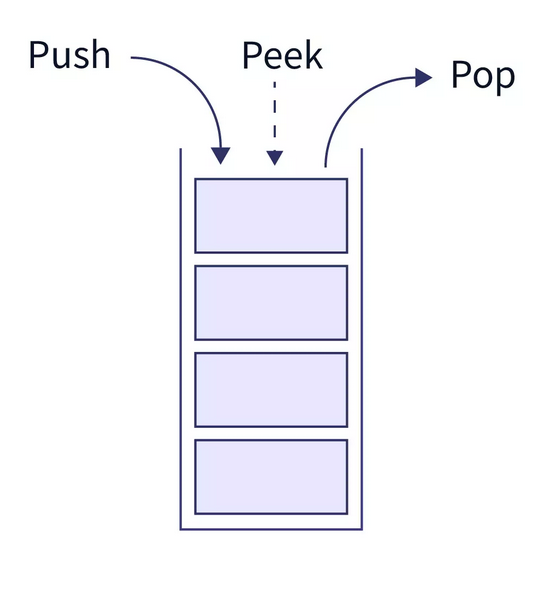
\includegraphics[width=0.5\textwidth]{stack}
            \caption{Source: \url{https://www.scaler.in/stack-operations/}}
        \end{figure}

    \end{columns}
\end{frame}

\begin{frame}{Stacks}{Operationer}
    \begin{columns}
        \column{.3\textwidth}
        \begin{minipage}{\textwidth}
            \scriptsize
            \begin{tcolorbox}
                
                \vspace{-\abovedisplayskip}
                \begin{codebox}
                    \Procname{$\proc{Stack-Empty}(S)$}
                    \li \If $\attrib{S}{top} \isequal 0$
                        \Then
                    \li     \Return True
                    \li \Else \Return False
                \end{codebox}
            \end{tcolorbox}

            \begin{tcolorbox}
                
                \vspace{-\abovedisplayskip}
                \begin{codebox}
                    \Procname{$\proc{Push}(S,x)$}
                    \li \If $\attrib{S}{top} \isequal \attrib{S}{size}$
                        \Then
                    \li \Error "overflow"
                    \li \Else
                    \li $\attrib{S}{top} \gets \attrib{S}{top} + 1$
                    \li $S[\attrib{S}{top}] \gets x$
                \end{codebox}
            \end{tcolorbox}

            \begin{tcolorbox}
                
                \vspace{-\abovedisplayskip}
                \begin{codebox}
                    \Procname{$\proc{Pop}(S)$}
                    \li \If $\proc{Stack-Empty}(S)$
                        \Then
                    \li \Error "underflow"
                    \li \Else
                    \li $\attrib{S}{top} \gets \attrib{S}{top} - 1$
                    \li \Return $S[\attrib{S}{top} + 1]$
                \end{codebox}
            \end{tcolorbox}
        \end{minipage}
    
        \column{.39\textwidth}

        Eksempel:

        \begin{itemize}
            \small
            \item Vi har stacken $S$ med $\attrib{S}{top} == 4$
            \item Vi kalder \proc{Push}($S, 17$) og $\proc{Push}(S,3)$
            \item Nu har vi $\attrib{S}{top} == 6$
            \item Vi kalder $\proc{Pop}(S)$
            \item Kaldet returnerer 3 og sætter $\attrib{S}{top} = 5$
            \item Bemærk at \alert{elementet stadig er i arrayet!}
        \end{itemize}

        \column{.3\textwidth}
        \begin{figure}[h]
            \centering
            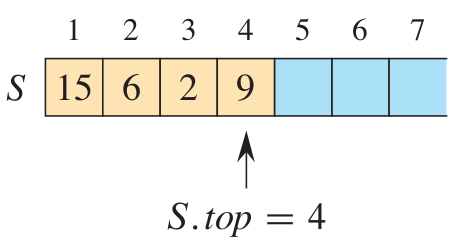
\includegraphics[width=0.8\textwidth]{stack-example/stack-a}
            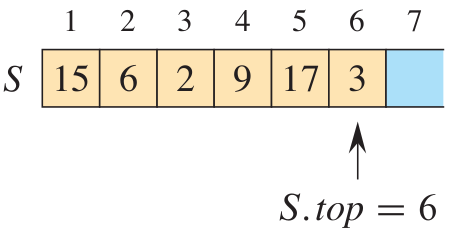
\includegraphics[width=0.8\textwidth]{stack-example/stack-b}
            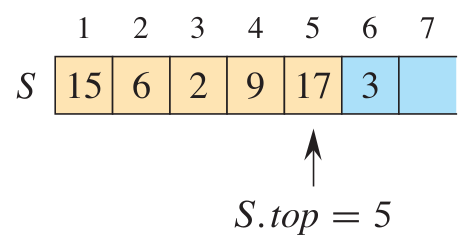
\includegraphics[width=0.8\textwidth]{stack-example/stack-c}
        \end{figure}

    \end{columns}
\end{frame}




\subsection{Linked Lists}

\subsection{Træer}

\section{Exercises}

\section{Heaps}

\subsection{En smart datastruktur}

\subsection{Heap sort}

\subsection{Priority Queues}




\begin{frame}{Dagens temaer}{Opsummering}
    \begin{itemize}
        \item Vi har mødt vores første sorteringsalgoritme --- Insertion-Sort!
            \begin{itemize}
                \item Simpel at implementere og forstå
                \item God til næsten sorterede sekvenser
                \item Den asymptotiske worst case køretid er kvadratisk
            \end{itemize}
        \item Loop invarianter og korrekthed
            \begin{itemize}
                \item Initialization, maintenance og termination
            \end{itemize}
        \item Asymptotisk analyse og notation
            \begin{itemize}
                \item $O, \Omega, \Theta$
            \end{itemize}
    \end{itemize}
\end{frame}


\begin{frame}{Tak for i dag!}{Flere exercises..}

    Den bedste måde ikke at snyde sig selv på er lave exercises!

    \begin{figure}[h]
        \centering
        
\includegraphics[width=0.8\textwidth]{exercises}
    \end{figure}
    
\end{frame}



\end{document}


